\documentclass{ueacmpstyle}

\RequirePackage{natbib}
\usepackage{graphicx,caption}
\usepackage{algorithm}
\usepackage{algpseudocode}
\usepackage{appendix}
\usepackage[hyphens]{url}
\graphicspath{ {./images/} }

\begin{document}
	\title{Developing Secure Systems Individual Report}
	\author{
		100203952 -- Thomas Mcloughlin\\
		CMP-6045B
	}
	\maketitle

    \section{Introduction}\label{sec:Intro}
    This report will present research of the top cyber threats and vulnerabilities of modern 
    systems with the aim of identifying methods to mitigate them.

    \section{Part 1}\label{sec:Pt1}
      % \cite{bibItem} << Example cite command (Look at overleaf tutorials) 
      % \ref{app:A} << This example references appendix A (Look at overleaf tutorials) 
      
      \subsection{Account Enumeration}\label{sub:AccEnum}
      Account enumeration is the manipulation of a service's login function to determine 
      the existence of a user. Attackers would determine this through two actions, first 
      by inputting a username and password into the login and if a message is received 
      stating that the password is wrong but not the username, then the attacker now 
      knows that the username exists. The way to mitigate this manipulation is to return 
      a generic message for a login failure not specifying whether the username or 
      password is wrong, however this mitigation can be nullified using the second method 
      where the attacker will try to log in and then compare the time taken to resolve the 
      failed login. If the response was quick then the username doesn't exist, if the 
      reponse took slightly longer then the service recognised the username and took longer 
      to try and match the password. This manipulation can also be mitigated by applying a 
      delay to the reponse when the username is wrong so that the attacker could not 
      tell the difference between the two responses.
      The mitigation methods described above fit into a secure by design approach because 
      they are concerned with the back end implementation details of the system and are 
      obscured well from any attackers. These techniques have been represented as 
      pseudocode in section \ref{sec:account-enumeration} of Appendix A.

      Threat actors likely to use account enumeration are attackers of any kind that could 
      range from casual programmers to criminal hackers trying to access various services. 
      A likely attack vector for using attack enumeration would be if the attacker had 
      gained access to a list of passwords for a service and was trying to find users to 
      match to so that they could break into the system.

      The interaction between the end users and the service will not be greatly affected 
      by the implementation of these mitigations with respect to the improved security 
      they provide, these mitigations do not affect the process of a sucessful login. 
      The only problem that can arise with usability will be that if a user forgets their 
      password or isn't sure what username they used for the service, the generic message 
      not specifying which is wrong can be frustrating and make logging in more difficult. 

      \subsection{Session Hijacking}\label{sub:SessHijk}
      Session hijacking is the utilisation of a lack of security given to website sessions 
      where a user that has logged in creates a session with the web server so that they 
      can make requests to the server without having to send log in details for every 
      request. These sessions have an attached ID so that the web server knows which user 
      it is communicating with, session hijacking refers to the multiple methods used to 
      gain access to a session, usually by accessing the ID. 

      When attempting to gain access using the ID, one possibility could be that the site 
      uses existent session ID's rather than generating a new ID for every session. This 
      opens up the session for attack from session fixation where the attacker uses a 
      known ID in a phishing email link to have the user login and authenticate themselves 
      then the attacker can hijack the session using the session ID \citep{OWASPSessionFixation}.

      There are multiple methods used to acquire session ID's to use for session fixation. 
      Session sniffing, the use of packet sniffing software to intercept session packets 
      and acquire the session ID attached to it, this can be done manually by the attacker 
      or the attacker may use malware to automate the process. The attacker may also brute 
      force the ID's by going through all possible permutations of the ID.

      The threat actors likely to use session hijackers are the same as stated above 
      in \ref{sub:AccEnum}. The risk posed by these attacks are: the attackers would 
      be able to gain access to a user authenticated login and perform any actions that the 
      user would be able to within that session such as a money transfer, the attacker would 
      also have access to any personal information that the session allows the user to view 
      which may lead to ID theft, the attacker may encrypt valuable/vital data for ransom 
      which could include intellectual property.

      The main methods to mitigate session hijacking attacks include: making session ID's 
      long and complex to avoid brute force access, make the site use a new session for 
      each time a user logs in and give each new session a unique ID to stop access if a 
      previously used ID has been compromised, ensure that a session is closed once a user 
      logs out or if the session is not being used and times out and finally, all session 
      data should be encrypted to prevent sniffing and malware attacks from accessing the 
      session ID's. Another method of mitigation extraneous to any technical measures 
      would include the training of end users to spot and avoid phishing emails.

      Generating a unique ID with enough complexity to avoid ID guessing is very important. 
      Therefore an example ID generation algorithm has been included as an acceptable 
      method shown in section \ref{sec:session-id-gen}. This algorithm was created using 
      recommended practices from \cite{OWASPSessionManagement} such as ensuring the entropy 
      number used is 64 bits to give an acceptable level of complexity.

      The addition of any of the mentioned mitigations would have very little affect on 
      the end users as the mitigations proposed are mainly secure by design techniques 
      that are more concerned with backend interaction. Usability will not be sacrificed 
      to a noticeable degree, the only affect on the user would be the requirement to 
      always log back into the system once they leave as the session they previously used 
      would have been closed.

      \subsection{SQL Injection}\label{sub:SqlInjection}
      SQL Injection is the manipulation of sql queries to interact with a database in 
      a way not intended by design, allowing the attacker to view, modify and delete 
      data from the database. These malicious queries are manipulated using input 
      fields such as the username and password inputs on a login page. If the login 
      input fields take any value inputted and inserts that input into an sql query 
      meant to retrieve user data, an example of which can be seen in section 
      \ref{sec:sql-query} of appedix A. If the attacker inputs part of a valid query 
      that will always evaluate to true, such as ' OR 1=1;--, then the example query 
      will return all user data from the table. Depending on how much sensitive data 
      is stored in the user table this could be a very dangerous breach, for example 
      if passwords were also stored in the user table.

      There are multiple methods of mitigation for sql injection that will be discussed 
      below. Firstly is the use of prepared statements where instead of inserting input 
      data into sql queries dynamically, the programmer defines all sql queries before-
      hand with inputs being parameterised. Any input then passed through to that query 
      avoids executing an unintended query and will instead take the entire input as a 
      string, for the example mentioned above using ' OR 1=1;-- the query would merely 
      search for a username matching the string "' OR 1=1;--" \citep{OWASPSqlInjectionPrevention}. 

      Secondly the use of stored procedures which act in a similar way to prepared 
      statements to avoid dynamic sql generation and instead parameterise and validate 
      input. The difference between the two is that stored procedures are sql queries 
      stored in the database that are then retrieved by the application when needed. 
      If implemented safely, avoiding the use of dynamic sql generation, then stored 
      procedures can provide nearly the same protection as prepared statements. 
      However a possible vulnerability of stored procedures comapared to prepared 
      statements would be in the case of a database requiring certain access levels 
      such as read and write permissions to prevent certain use of the database. In 
      the case of stored procedures, access to execute queries on the database is 
      required meaning that if an attacker were to gain access to the database then 
      they would have full execute privileges \citep{OWASPSqlInjectionPrevention}.

      Another method would be the implementation of whitelist validation for certain 
      parts of sql queries that cannot use bind variables as placeholders such as the 
      names of tables or columns. In this case if a user inputted parameter is used to 
      alter a queries target table or column then whitelist validation can be used to 
      avoid the risks of sql injection. By mapping input values to a preset whitelist 
      of possible choices for the target, the executed query avoids using the actual 
      input from the user, an example is described in section \ref{sec:whitelist-valid} 
      of appendix A.

      The mitigation methods discussed above would all be necessary inclusions in a 
      secure by design approach as it would take considerable effort to convert a system 
      to use these methods without a near full re-write of the related code. When trying 
      to combat sql injection attacks, mitigation should be considered from step 1 and not 
      be a reactionary change to a system.

      The threat actors likely to use sql injection are again the same as those stated 
      in \ref{sub:AccEnum}. The main risk of sql injection is that an attacker could be 
      able to execute any query they want on a database, in the case of a catastrophic 
      breach, the attacker could delete tables containing important data.

      End-users are unlikely to experience any adverse affects of the mitigation methods 
      as all methods used to prevent sql injection are backend related, these mitigations 
      would not affect usability of the system a noticeable amount to the common user. 
      The only affect on the system will be the minor performance concerns.

      \subsection{Cross-site Scripting}\label{sub:XSS}
      
        
    \section{Part 2}\label{sec:Pt2}


    \section{Conclusion}\label{sec:Con}

    
    \bibliographystyle{apalike}

	\bibliography{bibfile.bib}
	
	\newpage
	
	\appendix
	    % Using appendices in this format means you can just use \section{}
        \section{Appendix A}\label{app:A}   % Adding the label will allow you to reference this section in your work.

            \begin{figure}[ht]
              \subsection{Account Enumeration Mitigation}
              \label{sec:account-enumeration}
              \centering
              \begin{algorithm}[H]
              \caption{login(\emph{username}, \emph{password}) {\bf return} \emph{response}}
                \begin{algorithmic}[1]
                  \Require $username$, the username for login
                  \Require $password$, the password for login
                  \Require $users$, the set of users and passwords that the system will 
                            compare the login against
                  \Ensure \emph{response}, either a sucessful login or a response message
                  \State{$Failure \leftarrow$ "The username/password is incorrect"}
                  \ForAll{$user$ in $users$}
                    \If{$username$ = $user.username$}
                      \If{$password$ = $user.password$}
                        \State{$response \leftarrow Sucess$}
                        \Comment{Username and password correct}
                      \Else
                        \State{$response \leftarrow Failure$}  
                        \Comment{Username correct, password incorrect}
                      \EndIf
                    \Else
                    \State{$delay$} 
                    \Comment{Wait however long the check for the password would take}
                    \State{$response \leftarrow Failure$}
                    \Comment{Username and password incorrect}  
                    \EndIf
                  \EndFor
                  \State \Return $response$
                \end{algorithmic}
              \end{algorithm}
              \caption{Example of a login with account enumeration mitigation included}
              \label{fig:account-enumeration}
          \end{figure}

          \begin{figure}[ht]
            \subsection{Session ID Generation}
            \label{sec:session-id-gen}
            \centering
            \begin{algorithm}[H]
            \caption{generateUniqueSessionId() {\bf return} \emph{sessionId}}
              \begin{algorithmic}[1]
                \Require $IdList$, the set of existing session Id's
                \Require $prng$, pseudo random number generator
                \Ensure \emph{sessionId}, a unique session Id
                \State $entropy \leftarrow prng(64)$
                \Comment{Pseudo random number generation of length 64 bits}
                \State $Id \leftarrow generateId()$
                \Comment{Generate complex Id}
                \State $sessionId \leftarrow concatenate(Id, entropy)$
                \If{$sessionId \in IdList$}
                  \State generateUniqueSessionId()
                  \Comment{Session Id isn't unique, generate a new Id}
                \EndIf
                \State \Return $sessionId$
              \end{algorithmic}
            \end{algorithm}
            \caption{Example of a random session Id generator using recommended practices 
                      from \cite{OWASPSessionManagement}}
            \label{fig:session-id-gen}
          \end{figure}

          \begin{figure}
            \subsection{Basic User Retrieval SQL Query}
            \label{sec:sql-query}
            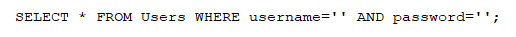
\includegraphics{basicSqlQuery}
            \caption{Example of a query that could be used to retrieve user data}
          \end{figure}

          \begin{figure}[ht]
            \subsection{Whitelist Validation Check}
            \label{sec:whitelist-valid}
            \centering
            \begin{algorithm}[H]
            \caption{getTableName(\emph{userInputValue}) {\bf return} \emph{outputTableName}}
              \begin{algorithmic}[1]
                \Require $userInputValue$, the value for the table name inputted by the user
                \Require $tableNameList$, list of valid table names
                \Ensure \emph{outputTableName}, the whitelisted chosen table name
                \ForAll{$name$ in $tableNameList$}
                  \If{$userInputValue$ = $name$}
                    \State $outputTableName$ = $name$
                  \EndIf
                \EndFor
                \State \Return $outputTableName$
                \Comment{\parbox[t]{.5\linewidth}{
                  if $outputTableName$ returns empty then we know that the user input was invalid
                }}
              \end{algorithmic}
            \end{algorithm}
            \caption{Example of table name validation, an adapted example from 
                     \cite{OWASPSqlInjectionPrevention}}
            \label{fig:whitelist-valid}
          \end{figure}

\end{document}
